\subsection*{\textcolor{subsectioncolor}{\textsf{4. \textit{TEST DESCRIPTION}}}}
\addcontentsline{toc}{subsection}{4. \textit{TEST DESCRIPTION}}


\subsubsection*{ServerSocket \& ClientSocket}

Konteks pengujian pada kedua modul ini adalah untuk membuktikan bahwa komunikasi antara subsistem \textit{server} dengan \textit{client} sudah dapat berjalan dengan lancar dan mapan.
Oleh karena itu,
antarmuka yang disediakan untuk pengujian ini cukup berupa konsol untuk memasukkan teks di sisi \textit{client} yang kemudian akan dikirim ke \textit{server},
dan sesampainya di \textit{server},
teks tersebut hanya akan dikembalikan lagi tanpa diolah terlebih dahulu.

Yang diuji dari ServerSocket adalah kemampuannya menyalakan layanan dan menunggu sampai ada \textit{client} dari manapun yang mencoba membuat sambungan dengan \textit{server},
kemampuannya mengenali informasi alamat \textit{client},
kemampuannya membuat \textit{server} berkomunikasi dengan satu \textit{client} tersebut setelah itu,
kemampuannya untuk membuat \textit{server} kembali menunggu setelah \textit{client} tersebut keluar dari sambungannya,
dan kemampuannya untuk mengulangi proses-proses tersebut ketika ada \textit{client} yang menyambung lagi.

Yang diuji dari ClientSocket adalah kemampuannya menyambung ke \textit{server},
kemampuannya mengenali \textit{server},
dan kemampuan untuk berkomunikasi dengannya.

Semua pengujian yang disebutkan di atas dilakukan pada jaringan yang keadaannya mapan.
Apa yang akan terjadi kalau keadaan jaringannya tidak mapan,
sebenarnya dapat juga diketahui hanya dengan simulasi.
Bagaimanapun, hal ini belum diuji karena akan memakan waktu yang tidak sebentar,
sedangkan masih banyak hal dalam pengembangan PUSPA yang harus didahulukan.

Masukan pada pengujian ini berupa teks seperti apa saja,
hanya saja karakter dengan banyak lebih daripada 100 tidak diharapkan,
karena penyangga yang disediakan di kedua modul hanya segitu besarnya (tanpa alasan tertentu).
Hal ini belum terlalu dipikirkan,
karena pada pelaksanaannya nanti memang karakter yang banyak sebagai masukan tidak diharapkan,
dan kemungkinan besar juga akan dibatasi oleh pemanfaatan bentuk suara, dan bukan teks, sebagai masukan (dan juga keluaran).
Keluaran pada pengujian ini juga berupa teks.

Peralatan perangkat keras pengujiannya melibatkan dua buah komputer.
Komputer pertama, bertindak sebagai server,
dan komputer kedua, bertindak sebagai client.
Konfigurasi pada pengujian ini adalah kedua komputer tersebut berada dalam satu LAN,
komputer \textit{server} dikenal dengan nama \texttt{rumahtenda.web.id},
dan \textit{port} yang digunakan adalah \textit{port} 12110.
Oleh karena itu, pada jaringannya harus dipastikan bahwa \textit{port} tersebut tidak terhalang.
Versi IP yang digunakan tidak ditentukan, sehingga dapat berupa versi 4 atau 6.
Untuk kenyamanan pengambilan gambar,
pada \textit{server}, peralatan perangkat lunaknya adalah \textit{server} SSH,
sedangkan pada \textit{client}, peralatannya mencakup \textit{client} SSH dan emulator terminal.
Hal ini dilakukan agar ServerSocket dapat dijalankan dari komputer \textit{client},
sehingga kedua modul dapat dijalankan dari satu komputer.
Untuk menjalankan ClientSocket, peralatan perangkat lunak yang dibutuhkan hanya emulator terminal.
Gambar \ref{ServerSocketConfiguration} menunjukkan konfigurasi pada \textit{server},
sedangkan Gambar \ref{ClientSocketConfiguration} menunjukkan konfigurasi pada \textit{client}.

\begin{figure}
\centering
\subfloat[\textit{Server}]{\label{ServerSocketConfiguration}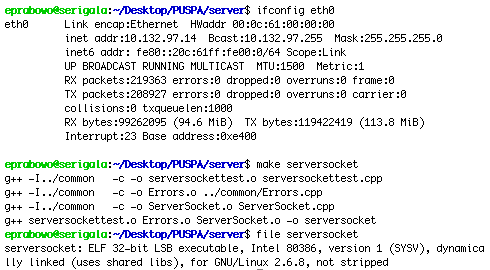
\includegraphics[width=0.5\textwidth]{ServerSocketConfiguration}}
\subfloat[\textit{Client}]{\label{ClientSocketConfiguration}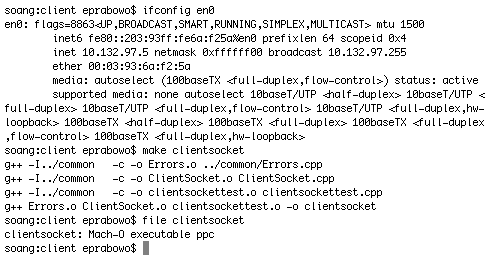
\includegraphics[width=0.5\textwidth]{ClientSocketConfiguration}}
\caption{Konfigurasi ServerSocket dan ClientSocket}
\label{SocketConfiguration}
\end{figure}

Hasil yang diharapkan dari pengujian ini adalah kedua modulnya dapat dengan lancar saling mengirim dan menerima data karakter,
dapat saling mengenali dengan baik melalui informasi mengenai alamat masing-masingnya,
dan kerja tiap modulnya tidak saling terpengaruhi oleh yang lain di saat salah satu memutuskan sambungan yang sudah terbangun.

Pengujian pertama adalah pengujian yang menyebabkan tidak adanya proses yang dilaksanakan.
Hal ini dapat dicapai dengan menyalakan hanya satu subsistem saja.
Gambar \ref{ServerSocketDegenerate} menunjukkan jalannya \textit{server} tanpa \textit{client},
sedangkan Gambar \ref{ClientSocketDegenerate} menunjukkan jalannya \textit{client} tanpa \textit{server}.

\begin{figure}
\centering
\subfloat[\textit{Server} tanpa \textit{client}]{\label{ServerSocketDegenerate}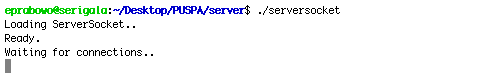
\includegraphics[width=0.5\textwidth]{ServerSocketDegenerate}}
\subfloat[\textit{Client} tanpa \textit{server}]{\label{ClientSocketDegenerate}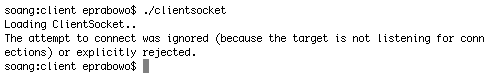
\includegraphics[width=0.5\textwidth]{ClientSocketDegenerate}}
\caption{\textit{Degenerate cases} pada ServerSocket dan ClientSocket}
\label{SocketDegenerate}
\end{figure}

Pengujian kedua adalah pengujian dengan memberikan nilai-nilai batas.
Satu hal yang masih memiliki nilai batas adalah penyangga yang digunakan untuk menampung karakter-karakter yang diterima melalui soket.
Pengujian ini dapat dilakukan dengan memberi masukan karakter yang banyaknya lebih daripada 100.
Gambar \ref{ServerSocketBoundary} menunjukkan \textit{server} saat menerima karakter-karakter yang banyak,
sedangkan Gambar \ref{ClientSocketBoundary} menunjukkan \textit{client} karakter-karakter banyak tersebut ketika dikirim dan ketika diterima kembali.

\begin{figure}
\centering
\subfloat[\textit{Server} menerima banyak karakter]{\label{ServerSocketBoundary}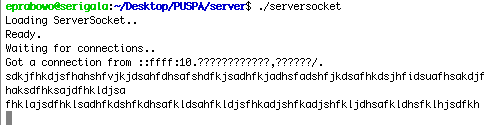
\includegraphics[width=0.5\textwidth]{ServerSocketBoundary}}
\subfloat[\textit{Client} mengirim banyak karakter]{\label{ClientSocketBoundary}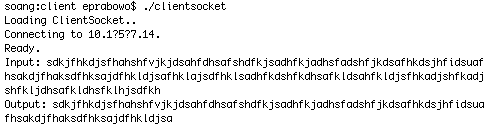
\includegraphics[width=0.5\textwidth]{ClientSocketBoundary}}
\caption{\textit{Boundary cases} pada ServerSocket dan ClientSocket}
\label{SocketBoundary}
\end{figure}

Pengujian ketiga adalah pengujian dengan memberikan data normal.
Gambar \ref{ServerSocketNonUnique} dan Gambar \ref{ClientSocketNonUnique} masing-masing menunjukkan \textit{server} dan \textit{client} saat menerima data normal.

\begin{figure}
\centering
\subfloat[\textit{Server} menerima data normal]{\label{ServerSocketNonUnique}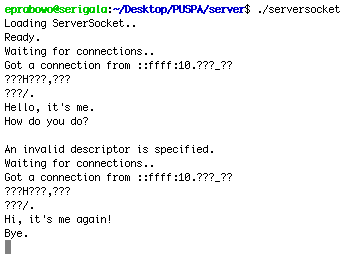
\includegraphics[width=0.5\textwidth]{ServerSocketNonUnique}}
\subfloat[\textit{Client} mengirim data normal]{\label{ClientSocketNonUnique}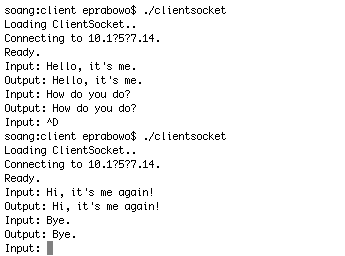
\includegraphics[width=0.5\textwidth]{ClientSocketNonUnique}}
\caption{\textit{Non-unique cases} pada ServerSocket dan ClientSocket}
\label{SocketNonUnique}
\end{figure}


\subsubsection*{DialogueManager}

Konteks pengujian pada modul ini adalah untuk membuktikan bahwa hubungan antara masukan dari pengguna dengan tanggapan yang dikeluarkan oleh modul ini sudah menyimulasikan suatu percakapan.
Di samping itu, pengujian ini juga sudah mulai mempertunjukkan pemenuhan prasyarat suatu pelaksanaan tugas,
walaupun pelaksanaannya belum dapat dilakukan karena hal tersebut merupakan tugas modul TaskManager.
Antarmuka yang disediakan untuk pengujian ini cukup berupa konsol untuk memasukkan teks dan keluarannya juga berupa teks.
Karena modul NaturalLanguageAnalyser yang mengolah bahasa manusia menjadi perwakilan makna untuk diolah oleh modul ini belum mapan,
dan karena modul NaturalLanguageGenerator yang harus mengolah tanggapan yang dihasilkan oleh modul ini menjadi bahasa manusia belum dikerjakan,
masukan dan keluaran modul ini untuk sementara masih dalam bentuk bahasa manusia.

Yang diuji dari modul ini adalah kemampuannya memberikan tanggapan yang cocok dengan masukan yang pengguna berikan,
kemampuannya menentukan \textit{communicative goals} dari percakapan yang sedang berlangsung,
dan kemampuannya melibatkan pengguna dalam pelaksanaan tugas yang diberikan oleh pengguna sendiri dengan cara menanyakan bagaimana pengguna menginginkan tugasnya dilaksanakan.

Yang belum diuji dari modul ini adalah pemeriksaan apakah masukan yang diberikan pengguna itu betul atau tidak dalam konteks percakapan yang sedang berlangsung.
Misalnya ketika pengguna ditanyakan mengenai suatu alamat surel,
jawaban yang diberikan pengguna belum diperiksa apakah betul atau tidak sebagai suatu alamat surel.

Masukan dan keluaran pada pengujian ini berupa teks,
dan banyaknya karakter yang dimasukkan tidak dibatasi.
Peralatan pengujiannya mencakup sebuah komputer dan sebuah emulator terminal.
Hasil yang diharapkan dari pengujian ini adalah simulasi percakapan.

Pengujian pertama adalah pengujian yang menyebabkan tidak adanya proses yang dilaksanakan.
Hal ini dapat dicapai dengan memberikan masukan berupa kata yang tidak diketahui maknanya oleh modul ini.
Gambar \ref{DialogueManagerDegenerate} menunjukkan pengujian ini.

\begin{figure}
\centering
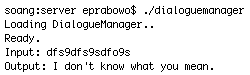
\includegraphics[width=0.5\textwidth]{DialogueManagerDegenerate}
\caption{\textit{Degenerate cases} pada DialogueManager}
\label{DialogueManagerDegenerate}
\end{figure}

Pengujian kedua adalah pengujian dengan memberikan data normal.
Gambar \ref{DialogueManagerNonUnique} menunjukkan simulasi percakapan yang dihasilkan saat yang dimasukkan adalah data normal.

\begin{figure}
\centering
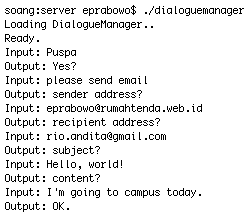
\includegraphics[width=0.5\textwidth]{DialogueManagerNonUnique}
\caption{\textit{Non-unique cases} pada DialogueManager}
\label{DialogueManagerNonUnique}
\end{figure}
